% $Id:
% !Mode:: "TeX:DE"    % Setting document mode and submode for WinEdt
% ..............................................................................
%             F I L M E  +  R O M A N E
% ~~~~~~~~~~~~~~~~~~~~~~~~~~~~~~~~~~~~~~~~~~~~~~~~~~~~~~~~~~~~~~~~~~~~~~~~~~~~~~
%
% Consider to add next time:
%  - Filme: Matrix, Tron, Echelon Verschwörung, ...
%  - Bücher: xxx, ...
% ~~~~~~~~~~~~~~~~~~~~~~~~~~~~~~~~~~~~~~~~~~~~~~~~~~~~~~~~~~~~~~~~~~~~~~~~~~~~~~


\begin{refsegment}

\newpage
\hypertarget{appendix-movies}{}
\section{Filme und belletristische Literatur mit Bezug zur Kryptographie}
\label{s:appendix-movies}
% {\bf Filme und Literatur mit Bezug zur Kryptographie} (siehe Anhang \ref{s:appendix-movies})
\index{Filme}
\index{Literatur}


Kryptographische Verfahren -- sowohl klassische wie moderne -- fanden auch
Eingang in die Literatur und in Filme. In manchen Medien werden diese nur
erwähnt und sind reine Beigabe, in anderen sind sie tragend und werden
genau erläutert, und manchmal ist die Rahmenhandlung nur dazu da, dieses
Wissen motivierend zu transportieren. Anbei der Beginn eines Überblicks.

% --------------------------------------------------------------------------
\subsection{Für Erwachsene und Jugendliche}
\label{s:Light-fiction-for-grownups}

%be_2005: Hatte zuerst \begin{thebibliography}{99999} und \bibitem[... ,
%         aber dann wurde immer der feste Titel "Literatur" bzw. "References"
%         geschrieben und wir fanden keine Möglichkeit, ihn weg zu bekommen.
%         Lösung: Stattdessen \begin{description} \item[...


\begin{description}

\item[\textrm{[Poe1843]}] \index{Poe 1843}
    Edgar Allan Poe\index{Poe, Edgar Allan}, \\
    {\em Der Goldkäfer}, 1843.\footnote{%
        Siehe \url{https://de.wikipedia.org/wiki/Der_Goldk%C3%A4fer}.

	Eine didaktisch aufbereitete Beschreibung zum Einsatz im Schulunterricht findet
        sich in Teil 1 der Artikelserie {\em RSA \& Co. in der Schule:
        Moderne Kryptologie, alte Mathematik, raffinierte Protokolle}.
        Siehe \cite{Witten1998}, S. 52 ff (\glqq Das Gold des Gehenkten\grqq).
	\index{RSA \& Co. in der Schule}

	Alle Materialien zu der Goldkäfer-Unterrichtsstunde (oder Doppelstunde)
	finden sich unter \url{http://www.informatik-im-kontext.de/} via
	\glqq E-Mail (nur?) für Dich\grqq~=> \glqq Vertraulichkeit mit Verschlüsselungsverfahren\grqq.
	% In den Materialien wird ein erprobter generischer Gang zu RSA präsentiert:
	% Monoalphabetische Verschlüsselung (Goldkäfer) => Knacken durch Häufigkeitsanalyse
	% => polyalphabetische Verschlüsselung => Knacken durch Bestimmung der Schlüssellänge (Kasiski, Friedman)
	% => One-Time-Pad als beweisbar sicheres Verschlüsselungsverfahren
	% => Problem des Schlüsselmanagments => asymmetrische Kryptographie (Diffie, Hellman, Merkle, RSA).

	Poe war nicht nur ein bekannter -- in seiner Heimat Amerika zunächst
	verkannter -- Schriftsteller und Erfinder des Kriminalromans,
	%% („Der Doppelmord in der Rue Morgue“, s. https://de.wikipedia.org/wiki/Edgar_Allan_Poe,
	%% https://de.wikipedia.org/wiki/Der_Doppelmord_in_der_Rue_Morgue)
	sondern auch ein begabter Kryptologe. Die Geschichte dazu wird auch in dem
	Krypto-Buch {\em Verschlüsselte Botschaften} \cite{Kippenhahn1997}
	erzählt.
    }\\
    Diese Kurzgeschichte erschien in Deutsch z.B. in der illustrierten und
    mit Kommentaren in den Marginalspalten versehenen Ausgabe "`Der Goldkäfer
    und andere Erzählungen"', Gerstenbergs visuelle Weltliteratur,
    Gerstenberg Verlag, Hildesheim, 2002.\\
    In dieser Kurzgeschichte beschreibt Poe als Ich-Erzähler seine
    Bekanntschaft mit dem sonderbaren Legrand. Mit Hilfe eines an der
    Küste Neuenglands gefundenen Goldkäfers, einem alten Pergament und
    den Dechiffrierkünsten von Legrand finden Sie den sagenhaften Schatz
    von Kapitän Kidd.\\
    Die Geheimschrift besteht aus 203 kryptischen Zeichen und erweist sich
    als allgemeine monoalphabetische Substitutions-Chiffre (vgl.
    Kapitel~\ref{monoalphabeticSubstitutionCiphers}). Ihre schrittweise
    Dechiffrie"-rung durch semantische und syntaktische Analyse
    (Häufigkeit der einzelnen Buchstaben in englischen Texten)
    wird in der Geschichte ausführlich erläutert.\footnote{%
      Teil der oben genannten Unterrichtsmaterialien ist auch ein Python-Programm.\index{Python}
      %% Außerdem gibt es eine schrittweise Lösung des Gold-Bug-Kryptogramms,
      %% das vor einigen Jahren Wittens Frau in Standard-HTML schrieb.
      Damit lässt sich das Kryptogramm mit Python {\em und} mit SageMath\index{SageMath}
      entschlüsseln.
      Siehe das Code-Beispiel in \ref{s:appendix-Code-for-light-fiction-books}.
      % \ref{Lit_Python-sample_Gold-bug}  Hier druckt er "A.1" ?
    }\\
    Der Entschlüsseler Legrand sagt darin (S. 39) den berühmten Satz:
    "`Und es ist wohl sehr zu bezweifeln, ob menschlicher Scharfsinn
    ein Rätsel ersinnen kann, das menschlicher Scharfsinn bei
    entsprechender Hingabe nicht wieder zu lösen vermag."'\\
    % D: Poe: 1809-1849, "Vater des Kriminalromans", er schloss Wetten ab,
    % dass er alle verschlüsselten Botschaften, die ihm Freunde und Leser
    % vorlegten, im Handumdrehen entschlüsseln könne. Gutes Gespür durch
    % viel Übung.
    % E: Poe, 1809-1849 was named "Father of the crime novel". He claimed,
    % that he will be able to decrypt any cipher sent to him by friends or
    % readers.
    %
    % Originalausgabe dieser illustrierten Ausgabe: "Le scarabée d'or et
    %                           autre nouvelles", Gallimard, Paris, 1998.
    % In "Der Goldkäfer" wird detailliert beschrieben, wie der verarmte
    % Hugenotte William Legrand in South Carolina die monoalphabetische
    % Geheimschrift des Piratenkapitäns Kidd knackt, die zu einem
    % sagenhaften Schatz führt.


\item[\textrm{[Verne1885]}] \index{Verne 1885}
    Jules Verne\index{Verne, Jules}, \\
    {\em Mathias Sandorf}, 1885. \\
    Dies ist einer der bekanntesten Romane des französischen Schriftstellers
    Jules Verne (1828-1905), der auch als "`Vater der Science Fiction"'
    bezeichnet wurde.\\
    Erzählt wird die spannende Geschichte des Freiheitskämpfers Graf
    Sandorf, der an die Polizei verraten wird, aber schließlich fliehen
    kann.\\
    Möglich wurde der Verrat nur, weil seine Feinde eine Geheimbotschaft an
    ihn abfangen und entschlüsseln konnten. Dazu benötigten sie eine
    besondere Schablone, die sie ihm stahlen. Diese Schablone bestand aus
    einem quadratischen Stück Karton mit 6x6 Kästchen, wovon 1/4, also neun,
    ausgeschnitten waren (vgl. die
    \hyperlink{turning-grille-cipher}{Fleißner-Schablone}
    in Kapitel~\ref{introsamplesTranspositionCiphers}).\\


    % Gefunden in: CRYPTO-GRAM, January 15, 2007, by Bruce Schneier
\item[\textrm{[Kipling1901]}] \index{Kipling 1901}
    Rudyard Kipling\index{Kipling, Rudyard}, \\
    {\em Kim}, 1901. \\
    Dieser Roman wird in der Besprechung von Rob Slade%
    \footnote{Siehe
      % \href{http://catless.ncl.ac.uk/Risks/24.49.html\#subj12} %% \ vor # nötig !
        \url{http://catless.ncl.ac.uk/Risks/24.49.html#subj12}.
    }
    folgendermaßen beschrieben:
    "`Kipling packte viele Informationen und Konzepte in seine Geschichten.
    In "`Kim"' geht es um das große "`Spiel"' Spionage und Bespitzelung.
    Schon auf den ersten 20 Seite finden sich Authentisierung über Besitz,
    Denial of Service, Sich-für-jemand-anderen-Ausgeben (Impersonation),
    Heimlichkeit, Maskerade, Rollen-basierte Autorisierung (mit
    Ad-hoc-Authentisierung durch Wissen), Abhören, und Vertrauen basierend
    auf Datenintegrität.
    Später kommen noch Contingency Planning gegen Diebstahl und
    Kryptographie mit Schlüsselwechsel hinzu."'\\
    Das Copyright des Buches ist abgelaufen.%
    \footnote{Sie können es lesen unter:\\
          \url{http://kipling.thefreelibrary.com/Kim} oder\\
          \url{http://www.readprint.com/work-935/Rudyard-Kipling}.
    }\\


\item[\textrm{[Doyle1905]}] \index{Doyle 1905}
    Arthur Conan Doyle\index{Doyle, Sir Arthur Conan}, \\
    {\em Die tanzenden Männchen}, 1905. \\
    In der Sherlock-Holmes-Erzählung {\em Die tanzenden Männchen}
    (erschienen erstmals 1903 im "`Strand Magazine"', und dann 1905 im
    Sammelband "`Die Rückkehr des Sherlock Holmes"' erstmals in Buchform)
    wird Sherlock Holmes mit einer Geheimschrift konfrontiert, die zunächst
    wie eine harmlose Kinderzeichnung aussieht. \\
    Sie erweist sich als monoalphabetische Substitutions-Chiffre (vgl.
    Kapitel~\ref{monoalphabeticSubstitutionCiphers}) des Verbrechers Abe
    Slaney. Holmes knackt die Geheimschrift mittels Häufigkeitsanaly"-se.\\


\item[\textrm{[Sayers1932]}] \index{Sayers 1932}
    Dorothy L. Sayers, \\
    {\em Zur fraglichen Stunde und Der Fund in den Teufelsklippen
    (Orginaltitel: Have his carcase)}, Harper, 1932 \\
    (Erste dt. Übersetzung {\em Mein Hobby: Mord} bei A. Scherz, 1964; \\
    dann {\em Der Fund in den Teufelsklippen} bei Rainer Wunderlich-Verlag,
    1974;\\
    Neuübersetzung 1980 im Rowohlt-Verlag). \\
    In diesem Roman findet die Schriftstellerin Harriet Vane eine Leiche
    am Strand und die Polizei hält den Tod für einen Selbstmord.
    Doch Harriet Vane und der elegante Amateurdetektiv Lord Peter Wimsey
    klären in diesem zweiten von Sayers's berühmten Harriet Vane's
    Geschichten den widerlichen Mord auf. \\
    Dazu ist ein Chiffrat zu lösen. Erstaunlicherweise beschreibt der
    Roman nicht nur detailliert die Playfair-Chiffre, sondern auch deren
    Kryptoanalyse (vgl. \hyperlink{playfair}{Playfair}
    in Kapitel~\ref{polygraphicSubstitutionCiphers}).\\


\item[\textrm{[Simmel1970]}] \index{Simmel 1970}
    Johannes Mario Simmel, \\
    {\em Und Jimmy ging zum Regenbogen}, Knaur Verlag, 1970. \\
    Der Roman spielt zwischen 1938 und
    1969 in Wien. Der Held Manuel Aranda deckt -- von mehreren Geheimdiensten
    verfolgt -- im Laufe der Handlung Stück für Stück die Vergangenheit seines
    ermordeten Vaters auf. Ein wichtiger Mosaikstein ist dabei ein
    verschlüsseltes Manuskript, das in Kapitel 33 entschlüssselt wird.
    Im Roman wird der Code als ein
    "`fünfundzwanzigfacher Caesar Code"' beschrieben, tatsächlich ist es eine
    Vigenère-Chiffre mit einem 25 Buchstaben langen Schlüssel. \\
    Das Buch wurde 1971 verfilmt.\\


\item[\textrm{[Crichton1988]}] \index{Crichton 1988}
    Michael Crichton, \\
    {\em Die Gedanken des Bösen (Orginaltitel: Sphere)}, Rororo, 1988. \\
    Ein Team verschiedener Wissenschaftler wird auf den Meeresgrund geschickt,
    um ein 900~m langes hoch entwickeltes Raumschiff zu untersuchen. Die
    Eigenheiten und psychischen Probleme der Forscher treten durch lebensbedrohliche
    Ereignisse und ihr Abgeschnittensein von oben immer mehr in den Vordergrund.
    Es gibt viele Rätsel: Das Raumschiff liegt schon 300 Jahre da, es hat
    englische Beschriftungen, es führt scheinbar ein Eigenleben, die menschliche
    Vorstellungskraft materialisiert sich. Unter anderem erscheint auf dem
    Bildschirm ein im Buch vollständig abgedruckter Code, der von dem genialen
    Mathematiker Harry entschlüsselt werden kann: ein einfacher spiralenförmiger
    Ersetzungscode.\\


\item[\textrm{[Seed1990]}] \index{Seed 1990}
    Regie Paul Seed (Paul Lessac), \\
    {\em Das Kartenhaus (Orginaltitel: House of Cards)}, 1990 (dt. 1992). \\
    In diesem Film versucht Ruth, hinter das Geheimnis zu kommen, das ihre
    Tochter verstummen ließ. Hierin unterhalten sich Autisten mit Hilfe von
    5- und 6-stelligen Primzahlen (siehe
    Kapitel~\ref{Chapter_Primes}).
    Nach über eine Stunde kommen im Film die folgenden beiden (nicht
    entschlüsselten) Primzahlfolgen vor:
%  \vskip -30pt  %be_2005 Bewirkt anscheinend nichts -- Abstand etwas zu groß.
    \begin{center}
    $21.383, \;\;176.081, \;\;18.199, \;\;113.933, \;\;150.377, \;\;304.523, \;\;113.933$\\
    $193.877, \;\;737.683, \;\;117.881, \;\;193.877$
    \end{center}
    \vskip +10 pt   % da "\\" hier nicht geht!


\item[\textrm{[Robinson1992]}] \index{Robinson 1992}
    Regie Phil Alden Robinson, \\
    {\em Sneakers - Die Lautlosen (Orginaltitel: Sneakers)},
    Universal Pictures Film, 1992. \\
    In diesem Film versuchen die "`Sneakers"' (Computerfreaks um ihren Boss
    Martin Bishop), den "`Bösen"' das Dechiffrierungsprogramm SETEC abzujagen.
    SETEC wurde von einem genialen Mathematiker vor seinem gewaltsamen Tod
    erfunden und kann alle Geheimcodes dieser Welt entschlüsseln.\\
    In dem Film wird das Verfahren nicht beschrieben%
    \footnote{
       An dem Film hatte Leonard Adleman (das "`A"' von RSA) als mathematischer
       Berater mitgearbeitet. Die recht lustige Geschichte über seine Mitwirkung
       bei Sneakers beschreibt er selbst auf seiner Homepage unter
       %% BE_8.8.18: Link tot: \url{http://www.usc.edu/dept/molecular-science/fm-sneakers.htm}.
       \url{http://world.std.com/~reinhold/math/sneakers.adleman.html}.
       Man kann man davon ausgehen, dass es sich bei dem überall benutzten
       Verschlüsselungsverfahren um RSA handelt.
       In dem Chip ist demnach ein bis dahin unbekanntes, schnelles
       Faktorisierungsverfahren\index{Faktorisierung} implementiert.
    }.\\


\item[\textrm{[Baldacci1997]}] \index{Baldacci 1997}
    David Baldacci, \\
    {\em Das Labyrinth. Total Control}, Lübbe, 1997. \\
    Jason Archer, Direktor einer Technologie-Firma, verschwindet plötzlich.
    Seine Frau Sidney Archer versucht, den Grund seines plötzlichen Todes
    herauszufinden, und entdeckt, wie das Finanzsystem missbraucht wird und
    dass die reale Macht bei denen mit dem meisten Geld liegt. Hier helfen
    dann auch gute Passworte nicht...\\


\item[\textrm{[Natali1997]}] \index{Natali 1997}
    Regie Vincenzo Natali, \\
    {\em Cube (Orginaltitel: Sneakers)},
    Mehra Meh Film, 1997. \\
    In diesem kanadischen Low-Budget-Film finden sich 7 sehr unterschiedliche
    Personen in einem endlos scheinenden Labyrinth von würfelartigen Räumen.\\
    Die Personen wollen nach draußen, müssen dazu aber die Räume durchqueren,
    von denen manche tödliche Fallen darstellen. Um herauszufinden, welche
    Räume gefährlich sind, spielt Mathematik eine entscheidende Rolle: Jeder
    Raum hat am Eingang eine Folge von 3 mal 3 Ziffern. Zuerst nehmen
    sie an, dass alle Räume Fallen sind, wo wenigstens eine der 3 Zahlen eine
    Primzahl ist. Später stellt sich heraus, dass auch alle diejenigen Räume
    Fallen sind, bei denen eine der 3 Zahlen eine Potenz von genau einer
    Primzahl ist (Fallen sind also $p^n$, z.B. $128=2^7$ oder
    $101 = 101^1 = prim$, aber nicht $517 = 11*47$).\\


\item[\textrm{[Becker1998]}] \index{Becker 1998}
    Regie Harold Becker, \\
    {\em Das Mercury Puzzle (Orginaltitel: Mercury Rising)},
    Universal Pictures Film, 1998. \\
    Die NSA hat einen neuen Code entwickelt, der angeblich weder von Menschen
    noch von Computern geknackt werden kann. Um die Zuverlässigkeit zu testen,
    verstecken die Programmierer eine damit verschlüsselte Botschaft in
    einem Rätselheft.\\
    Simon, eine neunjähriger autistischer Junge, knackt den Code.
    Statt den Code zu fixen, schickt ihm ein Sicherheitsbeamter einen Killer.
    Der FBI-Agent Art Jeffries (Bruce Willis) beschützt den Jungen und
    stellt den Killern eine Falle.\\
    Das Chiffrier-Verfahren wird nicht beschrieben.\\


\item[\textrm{[Brown1998]}] \index{Brown 1998}
    Dan Brown, \\
    {\em Diabolus (Orginaltitel: Digital Fortress)}, Lübbe, 2005. \\
    Dan Browns erster Roman "`The Digital Fortress"' erschien 1998 als E-Book,
    blieb jedoch damals weitgehend erfolglos.\\
    Die National Security Agency (NSA) hat für mehrere Milliarden US-Dollar
    einen gewaltigen Computer gebaut, mit dem sie in der Lage ist, auch nach
    modernsten Verfahren verschlüsselte Meldungen (natürlich nur die von
    Terroristen und Verbrechern) innerhalb weniger Minuten zu entziffern.\\
    Ein abtrünniger Angestellter erfindet einen unbrechbaren Code und
    sein Computerprogramm Diabolus zwingt damit den Supercomputer zu
    selbstzerstörerischen Rechenoperationen. Der Plot, in dem auch die
    schöne Computerexpertin Susan Fletcher eine Rolle spielt, ist ziemlich
    vorhersehbar.\\
    Die Idee, dass die NSA oder andere Geheimdienste jeden Code knacken
    können, wurde schon von mehreren Autoren behandelt: Hier hat der
    Supercomputer 3 Millionen Prozessoren -- trotzdem ist es aus heutiger
    Sicht damit auch nicht annäherungsweise möglich, diese modernen Codes
    zu knacken.\\


\item[\textrm{[Elsner1999]}] \index{Elsner 1999}
    Dr.~C.~Elsner, \\
    {\em Der Dialog der Schwestern}, c't, Heise-Verlag, 1999. \\
    In dieser Geschichte, die dem CrypTool-Paket\index{CrypTool} als PDF-Datei
    beigelegt ist, unterhalten sich die Heldinnen vertraulich mit einer
    Variante des RSA-Verfahrens (vgl. Kapitel~\ref{rsabeweis} ff.).
    Sie befinden sich in einem Irrenhaus unter ständiger Bewachung.\\


\item[\textrm{[Stephenson1999]}] \index{Stephenson 1999}
    Neal Stephenson, \\
    {\em Cryptonomicon}, Harper, 1999. \\
    Der sehr dicke Roman beschäftigt sich mit Kryptographie sowohl im
    zweiten Weltkrieg als auch in der Gegenwart.
    Die zwei Helden aus den 40er-Jahren sind der glänzende Mathematiker und
    Kryptoanalytiker Lawrence Waterhouse, und der übereifrige,
    morphiumsüchtige Bobby Shaftoe von den US-Marines.
    Sie gehören zum Sonderkommando 2702, einer Alliiertengruppe, die
    versucht, die gegnerischen Kommunikationscodes zu knacken und dabei
    ihre eigene Existenz geheim zu halten. \\
    In der Gegenwartshandlung tun sich die Enkel der Weltkriegshelden -- der
    Programmierfreak Randy Waterhouse und die schöne Amy Shaftoe -- zusammen. \\
    Cryptonomicon ist für nicht-technische Leser teilweise schwierig zu
    lesen. Mehrere Seiten erklären detailliert Konzepte der Kryptographie.
    Stephenson legt eine ausführliche Beschreibung der Solitaire-Chiffre
    (siehe Kapitel~\ref{Further-PaP-methods}) bei, ein
    Papier- und Bleistiftverfahren\index{Papier- und Bleistiftverfahren},
    das von Bruce Schneier entwickelt wurde und im
    Roman "`Pontifex"' genannt wird. Ein anderer, moderner Algorithmus
    namens "`Arethusa"' wird dagegen nicht offengelegt.\\


\item[\textrm{[Elsner2001]}] \index{Elsner 2001}
    Dr.~C.~Elsner, \nopagebreak\\
    {\em Das Chinesische Labyrinth}, c't, Heise-Verlag, 2001. \\
    In dieser Geschichte, die dem CrypTool-Paket\index{CrypTool} als PDF-Datei
    beigelegt ist, muss Marco Polo in einem Wettbewerb Probleme aus der
    Zahlentheorie lösen, um Berater des großen Khan zu werden. Alle Lösungen
    sind angefügt und erläutert.\\


\item[\textrm{[Colfer2001]}] \index{Colfer 2001}
    Eoin Colfer, \\
    {\em Artemis Fowl}, List-Verlag, 2001. \\
    In diesem Jugendbuch gelangt der junge Artemis, ein Genie und Meisterdieb,
    an eine Kopie des streng geheimen "`Buches der Elfen"'. Nachdem er es mit
    Computerhilfe entschlüsselt hat, erfährt er Dinge, die kein Mensch
    erfahren dürfte. \\
    Der Code wird in dem Buch nicht genauer beschrieben.\\


\item[\textrm{[Howard2001]}] \index{Howard 2001}
    Regie Ron Howard, \\
    {\em A Beautiful Mind}, 2001. \\
    Verfilmung der von Sylvia Nasar verfassten Biographie des
    Spieltheoretikers John Nash.
    Nachdem der brillante, aber unsoziale Mathematiker geheime kryptographische
    Arbeiten annimmt, verwandelt sich sein Leben in einen Alptraum. Sein
    unwiderstehlicher Drang, Probleme zu lösen, gefährden ihn und sein
    Privatleben.
    Nash ist in seiner Vorstellungswelt ein staatstragender Codeknacker. \\
    Konkrete Angaben zur seinen Analyseverfahren werden nicht beschrieben.\\


\item[\textrm{[Apted2001]}] \index{Apted 2001}
    Regie Michael Apted, \\
    {\em Enigma -- Das Geheimnis}, 2001. \\
    Verfilmung des von Robert Harris verfassten "`historischen Romans"'
    {\em Enigma} (Hutchinson, London, 1995) über die berühmteste
    Verschlüsselungsmaschine in der Geschichte, die in
    Bletchley Park nach polnischen Vorarbeiten gebrochen wurde.
    Die Geschichte spielt 1943, als der eigentliche Erfinder Alan Turing
    schon in Amerika war. So kann der Mathematiker Tom Jericho als Hauptperson
    in einem spannenden Spionagethriller brillieren.\\
    Konkrete Angaben zu dem Analyseverfahren werden nicht gemacht.\\


\item[\textrm{[Isau2003]}] \index{Isau 1997}
    Ralf Isau, \\
    {\em Das Museum der gestohlenen Erinnerungen}, Thienemann-Verlag, 1997/2003. \\
    Ein sehr spannender, hervorragend recherchierter und doch leicht zu lesender
    Roman mit einem tiefen Hintersinn.\\
    Als die Zwillinge Oliver und Jessica von ihren Ferien zurückkommen, haben sie
    ihren Vater vergessen. Die Realität verschiebt sich und niemand scheint es zu
    bemerken. An einigen Stellen bleiben manchmal Spuren zurück, die man
    entziffern kann.
    Zentrum der Geschichte ist das Ischtar-Tor im Berliner Pergamon-Museum.
    Nur mit dem Scharfsinn einer irischen Professorin (die gleichzeitig
    Computerexpertin, Archäologin und Philologin ist), den besonderen
    Beziehungen zwischen Zwillingen und den vereinten Kräften der
    Computergemeinschaft kann der letzte Teil des Spruches gelöst werden.\\
    Das Buch wurde als bestes Jugendbuch ausgezeichnet und liegt in 8 Sprachen vor.\\


\item[\textrm{[Brown2003]}] \index{Brown 2003}
    Dan Brown, \\
    {\em Sakrileg (Orginaltitel: The Da Vinci Code)}, Lübbe, 2004. \\
    Der Direktor des Louvre wird in seinem Museum vor einem Gemälde Leonardos
    ermordet aufgefunden, und der Symbolforscher Robert Langdon gerät in eine
    Verschwörung.\\
    Innerhalb der Handlung werden verschiedene klassische Chiffren (Substitution
    wie z.B. Caesar oder Vigen\`ere, sowie Transposition und Zahlencodes)
    angesprochen. Außerdem klingen interessante Nebenbemerkungen über
    Schneier oder die Sonnenblume an.
    Der zweite Teil des Buches ist sehr von theologischen Betrachtungen
    geprägt. \\
    Das Buch ist einer der erfolgreichsten Romane der Welt.\\

% Rezensionen aus der Amazon.de-Redaktion:
% Bestsellerautor Dan Brown bietet mit Sakrileg erneut spannende und intelligente Unterhaltung vom Feinsten. Der Direktor des Louvre wird in seinem Museum vor einem Gemälde Leonardos ermordet aufgefunden, und der Symbolforscher Robert Langdon gerät ins Fadenkreuz der Polizei, war er doch mit dem Opfer just zur Tatzeit verabredet. Eine Verschwörung ist immer noch das Schönste. Stimmt, wenn sie schriftstellerisch so überzeugend und raffiniert inszeniert ist, wie es dem Amerikaner Dan Brown in diesem Thriller gelingt. Genaue Recherchen an den Schauplätzen und penible historische Studien in Zusammenarbeit mit seiner Frau Blythe, einer Kunsthistorikerin, machen das umfangreiche Werk nicht nur für Historiker und Religionswissenschaftler, sondern gerade auch für ein großes Publikum zu einem echten Vergnügen. Der Symbolologe Robert Langdon sitzt in der Klemme. Er gilt als Hauptverdächtiger im Fall Jacques Saunière, des ermordeten Direktors des Louvre, und gerät als solcher in die Fänge von Capitaine Bezu Fache, der als überaus gerissener Ermittler gilt. Saunière hatte im Todeskampf einen Hinweis auf Langdon gegeben. Mithilfe von Sophie Neveu, der Enkelin des Ermordeten, gelingt Langdon die Flucht. Beide sind der Überzeugung, dass Saunière vielmehr Informationen über eine Verschwörung des Opus Dei und der katholischen Kirche liefern wollte. Im Verlauf einer atemlosen Flucht von Frankreich nach England haben Langdon und Neveu knifflige Codes zu knacken, um Saunières Geheimnis zu lüften, der sich als Großmeister der Geheimorganisation Prieuré de Sion entpuppt. Auf ihren Fersen befindet sich nicht nur die Polizei. Die Handlung einer Nacht und eines Tages auf 600 fesselnden Seiten, die überdies Lust machen auf mehr Informationen zu Templern, Prieuré de Sion, Opus Dei sowie auf mehr historische Fakten -- was will man mehr. Und wer das Ganze nicht allzu ernst nimmt, wird die Lektüre sehr genießen -- am besten innerhalb einer Nacht und eines Tages.
% --Ulrich Deurer



\item[\textrm{[McBain2004]}] \index{McBain 2004}
    Scott McBain, \\
    {\em Der Mastercode (Orginaltitel: Final Solution)}, Knaur, 2005. \\
    In einer nahen Zukunft haben Politiker, Militärs und Geheimdienstchefs
    aus allen Staaten in korrupter Weise die Macht übernommen. Mit einem
    gigantischen Computernetzwerk names "`Mother"' und vollständiger
    Überwachung wollen sie die Machtverteilung und Kommerzialisierung für
    immer festschreiben.
    Menschen werden ausschließlich nach ihrem Kredit-Rating bewertet und
    global agierende Unternehmen entziehen sich jeder demokratischen
    Kontrolle.
    Innerhalb des Thrillers wird die offensichtliche Ungerechtigkeit,
    aber auch die realistische Möglichkeit dieser Entwicklung immer wieder
    neu betont.\\
    In den Supercomputer "`Mother"' wurde m.H. eines Kryptologen ein Code zur
    Deaktivierung eingebaut: In einem Wettrennen mit der Zeit versuchen
    Lars Pedersen, Oswald Plevy, die amerikanische Präsidentin, der britische
    Regierungschef und eine unbekannte Finnin namens Pia, die den Tod ihres
    Bruders rächen will, den Code zur Deaktivierung zu starten. Auf der
    Gegenseite agiert eine Gruppe mörderischer Verschwörer unter Führung
    des britischen Außenministers und des CIA-Chefs.\\
    Die englische Originalfassung "`The Final Solution"' wurde als Manuskript
    an Harper Collins, London verkauft, ist dort aber nicht erschienen.\\

	
\item[\textrm{[Burger2006]}] \index{Burger 2006}
    Wolfgang Burger, \\
    {\em Heidelberger Lügen}, Piper, 2006. \\
    In diesem Kriminalroman mit vielen oft
    unabhängigen Handlungssträngen und lokalen Geschichten geht es vor
    allem um den Kriminalrat Gerlach aus Heidelberg. Auf S. 207 f. wird aber
    auch der kryptologische Bezug von einem der Handlungsstränge kurz
    erläutert: der Soldat Hörrle hatte Schaltpläne eines neuen digitalen
    NATO-Entschlüsselungsgerätes kopiert und der Ermordete hatte versucht,
    seine Erkenntnisse an die Chinesen zu verkau"-fen.\\
    % siehe: www.wolfgang-burger.com


\newpage
\item[\textrm{[Vidal2006]}] \index{Vidal 2006}
    Agustin Sanchez Vidal, \\
    {\em Kryptum}, Dtv, 2006. \\
    Der erste Roman des spanischen Professors der Kunstgeschichte ähnelt
    Dan Browns "`Sakrileg"' aus dem Jahre 2003, aber angeblich hat Vidal schon
    1996 begonnen, daran zu schreiben. Vidals Roman ist zwischen historischem
    Abenteuerroman und Mystery-Thriller angesiedelt und war in Spanien ein
    Riesenerfolg.\\
    Im Jahre 1582 wartet Raimundo Randa, der sein Leben lang einem Geheimnis
    auf der Spur war, im Alkazar auf seinen Inquisitionsprozess.
    Dieses Geheimnis rankt sich um ein mit kryptischen Zeichen beschriftetes
    Pergament, von dem eine mysteriöse Macht ausgeht.
    Rund 400 Jahre später kann sich die amerikanische Wissenschaftlerin Sara
    Toledano dieser Macht nicht entziehen, bis sie in Antigua verschwindet.
    Ihr Kollege, der Kryptologe David Calderon, und ihre Tochter Rachel machen
    sich auf die Suche nach ihr und versuchen gleichzeitig, den Code zu knacken.
    Aber auch Geheimorganisationen wie die NSA sind hinter dem
    Geheimnis des "`letzten Schlüssels"' her. Sie sind bereit, dafür
    über Leichen zu gehen.\\
    % Korrekte Schreibweise ? :  Augustín Sánchez Vidal, David Calderón


% \vskip +30 pt   % damit Larsson auf einer neuen Seite beginnt
\item[\textrm{[Larsson2007]}] \index{Larsson 2007}
    Stieg Larsson, \\
    {\em Verdammnis (Originaltitel: Flickan som lekte med elden)}, Heyne, 2007. \\
    Der Autor wurde 2006 postum mit dem Skandinavischen Krimipreis als bester
    Krimiautor Skandinaviens geehrt. Die Superheldin Lisbeth Salander nutzt PGP
    und beschäftigt sich nebenbei auch mit mathematischen Rätseln wie dem Satz
    von Fermat.\\


\item[\textrm{[Preston2007]}] \index{Preston 2007}
    Douglas Preston, \\
    {\em Der Canyon (Orginaltitel: Tyrannosaur Canyon)}, Knauer, 2007. \\
    Ein spannender Thriller, bei dem es auch darum geht, warum die Dinosaurier
    ausstarben.

    Archäologe Stem Weathers wird im Labyrinth-Canyon erschossen. Noch bevor der
    Mörder ihn ausrauben kann, übergibt er sein Notizbuch an Tom Broadbent, einen
    dortigen Tierarzt, der zufällig vorbei kommt.

    In dem Notizbuch stehen auf 60 Seiten nur Ziffern. Deshalb bringt Tom es zu dem
    Ex-CIA-Kryptoanalytiker Wyman Ford, der sich in ein nahegelegenes Wüstenkloster
    zurückzog, nachdem seine Frau bei einem Einsatz getötet wurde.
    Zuerst lehnt Wyman jede Unterstützung ab und bezeichnet selbst gebastelte Codes
    als "`Idiotenchiffren"' -- von einem Idioten ausgedacht, von jedem Idioten zu
    entziffern. Mit dem Notizbuch verhält es sich aber nicht ganz so einfach. Nach
    intensiver Kryptoanalyse findet er heraus, dass die Ziffern keinen Code
    darstellen, sondern dass es der Output eines Bodenradargeräts mit dem Bild
    eines gut erhaltenen Tyrannosaurus Rex ist.

    Nach rund 250 Seiten gibt es eine überraschende Wende bei den endlosen
    Verfolgungsjagden: Masago, Chef einer sogenannten Black-Detachment-Einheit der CIA,
    kommt ins Spiel. Er erklärt: Waffen, die einmal erfunden wurden, werden immer auch
    eingesetzt. Die Menschheit wird sich ausrotten, aber seine Aufgabe sei es, das
    möglichst weit hinauszuzögern. Als Leiter der Abteilung LS480 will er mit allen
    Mitteln verhindern, dass Terroristen Zugang zu neuen gefährlichen biologischen
    Waffen erhalten.

    Der Mörder von Weathers hatte beim Durchsuchen der Leiche nur ein paar Gesteinsproben
    gefunden und mitgenommen. Diese wurden dann von einer jungen Forscherin namens Melodie
    Crookshank untersucht, ohne dass sie weiß, woher diese kommen. Sie findet darin eine
    besondere Virenform, die anscheinend eine außerirdische Lebensform darstellt.\\


\item[\textrm{[Twinig2008]}] \index{Twinig 2008}
    James Twinig, \\
    {\em Die schwarze Sonne (Orginaltitel: The Black Sun)}, Bastei Lübbe, 2008. \\
    Ein historisch-basierter Thriller mit einigen konstruierten Elementen, bei dem
    es auch darum geht, an das versteckte Uran der Nazis zu kommen, natürlich um die
    Menschheit zu retten ...

    Helden sind Tom Kirk, ein in London lebender Ex-CIA-Agent und früherer Kunstdieb,
    und Dominique de Lecourt -- sie liebt Herausforderungen inklusive Rätsel und Codes.

    Die einzigen kryptographischen Elemente sind ein "`Sprungcode"' (die Verbrecher
    nutzen das Verfahren zur Kommunikation via Zeitungsanzeigen), Steganographie
    (um die Enigma-Einstellungen zu verstecken), und eine Enigma-Nachricht (in der die
    Koordinaten des "`Schatzes"' verschlüsselt sind).

    Zu Beginn wird eine Enigma mit hohem Aufwand gestohlen, was notwendig ist,
    um die angelegte Handlung so zustande kommen zu lassen. In der Realität
    wäre heutzutage ein solcher Diebstahl völlig überflüssig, da es inzwischen
    hervorragende Software-Emulationen für die Enigma gibt ... \\


\item[\textrm{[Schröder2008]}] \index{Schröder 2008}
    Rainer M. Schröder, \\
    {\em Die Judas-Papiere}, Arena, 2008. \\
    "`Historienthriller"': Lord Pembroke hat im Jahre 1899 drei Männer und eine Frau
    in der Hand und beauftragt sie, die verschlüsselten Botschaften in dem Notizbuch
    seines verstorbenen Bruders Mortimer zu entschlüsseln und das Judas-Evangelium
    zu finden, das das Ende der Christenheit einläuten könnte. Dazu müssen sie
    Rätsel an vielen Orten der Welt lösen.
    Im Buch finden sich klassische Verfahren wie Polybius (S. 195) oder die
    Freimaurer-Chiffre (S. 557).\\


\item[\textrm{[Hill2009]}] \index{Hill 2009}
    Tobias Hill, \\
    {\em Der Kryptograph (Orginaltitel: The Cryptographer)}, C. Bertelsmann, 2009. \\
    London 2021: Die Firma SoftMark hat eine elektronische Währung entwickelt
    und etab"-liert, die durch einen nicht entschlüsselbaren Code allen Nutzern
    höchste Sicherheit garan"-tiert.
    Der Erfinder und Firmengründer John Law, wegen seiner mathematischen Begabung
    auch der Kryptograph genannt, ist damit zum reichsten Mann der Welt geworden.
    Doch dann wird der Code geknackt, und in einer dadurch verursachten
    Weltwirtschaftskrise geht auch die Firma von John Law pleite. Außerdem wird
    die Steuerfahnderin Anna Moore auf ihn angesetzt.\\


\item[\textrm{[Eschbach2009]}] \index{Eschbach 2009}
    Andreas Eschbach,\\
    {\em Ein König für Deutschland}, Lübbe, 2009.\\
    Der Roman dreht sich um die Manipulierbarkeit von Wahlcomputern.\\
    Vincent Merrit, ein junger US-amerikanischer Programmierer, wird erpresst,
    ein solches Programm zu schreiben. Neben kommerziell orientierten Erpressern
    kommen z.B. auch Online-Rollenspiele und Live-Rollenspiele (LARPs) in dem Roman vor.
    Weil Merrit den Missbrauch seines Programms ahnte, baute er eine Hintertür
    ein: Nimmt eine Partei namens VWM an der Wahl teil, erhält sie automatisch
    95 \% der Stimmen ...\\
    Die fiktive Handlung des Romans beruht auf zahlreichen überprüfbaren und
    genau recherchierten Tatsachen, auf die in Fußnoten hingewiesen wird.\\
    Während die kryptographischen Protokolle sicher gemacht werden können,
    bleiben ihre Implementierung und ihre Organisation anfällig gegen Missbrauch.\\


\item[\textrm{[Juels2009]}] \index{Juels 2009}
    Ari Juels,\\
    {\em Tetraktys}, Emerald Bay Books, 2009 (bisher nur in Englisch).\\
    Die Geschichte deckt die Verwundbarkeit der computer-basierten Identitäten und
    Sicherheiten auf, indem sie moderne Kyptographie mit klassischer Wissenschaft und
    Literatur verbindet.
    Der Kryptograph und Altphilologe Ambrose Jerusalem ist Abgänger der UC Berkeley
    mit einer schönen Freundin und einer aussichtsreichen Zukunft, bis ihn die NSA
    rekrutiert, um eine Serie mysteriöser Computereinbrüche zu verfolgen. Viele kleine
    Puzzlestücke lassen vermuten, dass jemand die RSA-Verschlüsselung gebrochen hat.
    Hinter den Angriffen scheint ein geheimer Kult zu stecken, Anhänger von Pythagoras,
    dem großen griechischen Mathematiker und Philosophen, der glaubte, die Wirklichkeit
    könne nur mit Hilfe eines mystischen Zahlensystems verstanden werden.\\
    % http://www.tetraktysnovel.com/
    % http://www.thenervousbreakdown.com/ajuels/2009/12/tetraktys-an-excerpt/
    % http://www.amazon.com/Tetraktys-Ari-Juels/dp/0982283709


\item[\textrm{[Suarez2010]}] \index{Suarez 2010}
    Daniel Suarez, \\
    {\em Daemon: Die Welt ist nur ein Spiel (Orginaltitel: Daemon)}, rororo, 2010. \\
    Dies gilt als eines der spannendsten Bücher der letzten Jahre -- ein Near-Science
    Fiction-Thriller, der die Entwicklungen in der realen Welt und die Möglichkeiten von
    aktuellen Forschungen wie denen von Google-X-Labs (Google-Brille, selbst-steuernde
    Autos, 3-D-Drucker, ...) in einer plausiblen Geschichte vereint.

    Nach dem Tod des Computergenies und Spieleentwicklers Matthew Sobol agiert ein Daemon
    im Internet, der scheinbar skrupellos immer mehr Menschen und Firmen geschickt
    manipuliert und ausbildet.

    Durch die Beherrschung der Daten ist ihm jeder ausgeliefert. Die Kommunikation seiner
    Söldner ist geprägt von High-Tech und Verschlüsselung -- ebenso die Kommunikation der
    verteilten Instanzen seiner Inkarnation. Kern ist ein MMORPG-Spiel (Massive
    Multiplayer Online Role-Playing Game), das stark an WoW erinnert. Auch hierin gibt es
    verschlüsselte Botschaften, z.B. um die besten Spieler anzuwerben:\\
	m0wFG3PRCoJVTs7JcgBwsOXb3U7yPxBB

    Die Handlung ist wiederholungsfrei, komplex, vielfältig, sehr spannend und enthält mit
    ihrer Kritik an den Plutokraten auch konkrete gesellschaftskritische Elemente.
    Das Ende ist offen. Und die Ideen scheinen realisierbar in allernächster Zukunft ...\\

   % [[[ Vielfältige gute Besprechungen für den Daemon:
   %     http://www.phantastik-couch.de/daniel-suarez-daemon-die-welt-ist-nur-ein-spiel.html
   %     --> SEHR gute Besprechung.
   %     http://www.phantastik-couch.de/daniel-suarez-darknet.html
   %     http://www.amazon.de/DARKNET-Daniel-Suarez/dp/3499252449
   %     http://www.rowohlt.de/magazin_artikel/Daniel_Suarez_Darknet.2943165.html
   %     http://www.literatopia.de/index.php?option=com_content&view=article&id=11130:darknet&catid=68:thriller&Itemid=100
   %     http://www.hr-online.de/website/specials/buchmesse2011/index.jsp?rubrik=67905&key=standard_rezension_42501444
   %     http://www.avameo.de/index.php/2012/05/01/konvergenz-thriller-daemon-und-darknet-von-daniel-suarez/
   % ]]]



\item[\textrm{[Olsberg2011]}] \index{Olsberg 2011}
    Karl Olsberg,\\
    {\em Rafael 2.0}, Thienemann Verlag, 2011, 240 Seiten.\\
    Michael und Rafael Ogilvy sind begabte Zwillinge, die sich sehr gut verstehen.
    Bevor der unheilbar kranke Rafael stirbt, entwickelt sein Vater ein virtuelles
    Computer-Ebenbild von ihm, eine künstliche Intelligenz (KI). Das ist ein gut
    gehütetes Geheimnis, bis Michael eines Tages dahinter kommt, was sein Vater da vor
    ihm versteckt. Sein erstes Entsetzen verwandelt sich jedoch bald in Freude.
    So hat er noch etwas, das ihn an seinen Bruder erinnert.\\
    Doch dieses Computersystem ist auch für das Militär interessant.
    Eines Tages wird Michaels Vater entführt und die
    Firma und somit auch das Computerprogramm Rafael 2.0 geraten in die falschen Hände.
    Michael wird von seinem Onkel in ein Internat verbannt, aus dem er aber fliehen kann.
    Fortan versuchen Michael und seine Freunde alles, um seinen Vater zu finden, von dem
    sie annehmen, dass er von einer konkurrierenden Firma entführt wurde. Ab hier wird
    die Geschichte richtig spannend ...
    Michael erfährt, dass es eine weitere künstliche Intelligenz, Metraton, gibt,
    die den Menschen nicht so wohlgesonnen ist.
    Nichts wird zu sehr vertieft, junge Jugendliche sind die Zielgruppe.
    Trotzdem entsteht auch Tiefgang, wenn es bspw. um Machenschaften bei Firmenübernahmen
    geht.\\
    Aus kryptologischer Sicht: Spannend ist der Abschnitt zur Faktorisierung: Mit einer
    Variante kann Michael erkennen, ob der Computer betrügt ...\\
    %% \glqq x\grqq~
    %% ``x''



\item[\textrm{[Burger2011]}] \index{Burger 2011}
    Wolfgang Burger, \\
    {\em Der fünfte Mörder}, Piper, 2011. \\
    Ort \& Zeit der Handlung: Deutschland / Heidelberg, 1990 - 2009.
    Folge 7 der Alexander-Gerlach-Serie.
    Beinahe wäre Kriminaloberrat Alexander Gerlach (Ich-Erzähler) Opfer eines
    Bombenanschlags geworden, als der Geländewagen eines bulgarischen Zuhälters explodiert.
    Als Gerlach ermittelt, weil er einen Bandenkrieg verhindern will, wird er von oberster
    Stelle zurückgepfiffen.
    Journalist Machatschek unterstützt Gerlach, tauscht mit ihm Informationen aber nur
    per Skype und einem Zusatzprogramm dazu aus, da er nur das für abhörsicher hält.\\
    % S. 172



\item[\textrm{[Suarez2011]}] \index{Suarez 2011}
    Daniel Suarez, \\
    {\em Darknet (Orginaltitel: Freedom (TM))}, rororo, 2011. \\
    Dies ist der erschreckend plausible Nachfolger zu "`Daemon"' (siehe oben).
    Gleich zu Beginn werden einige offene Fäden aus dem ersten Buch aufgenommen und
    geklärt. Die Beschreibungen sind direkter, die Charaktere werden ausgearbeitet,
    insbesondere Loki. Nachdem in "`Daemon"' die Grundlagen gelegt wurden, nutzt Suarez
    dies, um ein neues Konzept gesellschaftlicher Organisation zu erläutern, die
    durch Informationstechnologie neue Fähigkeiten erlangt. Dabei werden die Motive
    deutlich, die sowohl die alten Potentaten als auch die neue Daemon-Gesellschaft
    treibt, die sich noch während der Geschichte stark weiter entwickelt.
    Kryptographie wird in diesem Buch als ein natürlicher Teil der modernen Technologie
    und der modernen Kriegsführung beschrieben.
    Die neue Gesellschaft in "`Darknet"' basiert auf dem Darknet,
    einer Alternative zum Internet, aufgebaut auf schnellen drahtlosen Meshnetzen, die
    eine sehr hohe Standfestigkeit und Verfügbarkeit haben. Auch wenn die Geschichte
    in einigen Teilen schockierend ist, scheint sie realistisch und nicht weit weg
    von der simultanen Nutzung moderner Technologie, die unser aller Leben durchdringt
    als virtuelle Welt, die sich über die reale Welt legt.\\
   % [[[Gute Besprechung zum Nachfolgebuch: Freedom = Darknet
   %    http://www.goodreads.com/book/show/7132363-freedom-tm]]]



\item[\textrm{[Eschbach2011]}] \index{Eschbach 2011}
    Andreas Eschbach, \\
    {\em Herr aller Dinge}, Lübbe, 2011. \\
    Dieser Roman hätte es verdient, viel bekannter zu werden: Die Idee darin des
    \glqq schrecklichsten aller Verbrechen\grqq, die der Grund der ganzen Geschichte
    wird, ist neu und geradzu revolutionär, aber auch unendlich traurig.
    Anhand der scheiternden Paarbeziehung von Hiroshi (Erfindergenie) und Charlotte
    werden große Themen wie Gerechtigkeit, Wohlstand und Macht behandelt.\\
    Aus kryptographischer Sicht: Hiroshi benutzt verteilte Berechnung und hat
    ein Verschlüs\-se\-lungs- und Backup-System entwickelt, dass die Regierung,
    die ihn verwanzt, in die Irre leitet.\\
    % Master of the universe -- master of all staff



\item[\textrm{[Elsberg2012]}] \index{Elsberg 2012}
    Marc Elsberg,\\
    {\em Blackout -- Morgen ist es zu spät}, Blanvalet, 2012, 800 Seiten.\\
    An einem kalten Wintertag brechen in Europa alle Stromnetze zusammen.
    Die Behörden, Stromversorger und Sicherheitsfirmen tappen im Dunkeln und können das
    Problem nicht beheben.
    Der italienische Informatiker Piero Manzano vermutet, dass hier Terroristen mit
    Hilfe von Hackern angreifen: In den bei
    allen Abnehmern eingesetzten Smart-Metern, Software-gesteuerten Stromzählern, wurde
    die Software manipuliert. Die Sicherheits- und Verschlüsselungskomponenten wurden
    geknackt, so dass Fremde sie mit falschen Steuerungsbefehlen außer Betrieb setzen
    konnten. Die erschreckenden Folgen an den unterschiedlichen Orten sind realistisch
    und spannend erzählt. Ebenso die Reaktionen der Menschen ...\\



\item[\textrm{[Olsberg2013]}] \index{Olsberg 2013}
    Karl Olsberg,\\
    {\em Die achte Offenbarung}, Aufbau Taschenbuch, 2013, 460 Seiten.\\
    Kann eine Botschaft aus der Vergangenheit unsere Zukunft verändern?
    Dem Historiker Paulus Brenner fällt ein uraltes, verschlüsseltes Manuskript aus
    dem Besitz seiner Familie in die Hände. Doch je mehr er von dem Text dekodiert,
    desto rätselhafter wird der Inhalt: Denn das Buch sagt mit erstaunlicher Präzision
    Ereignisse voraus, die zum Zeitpunkt seiner vermuteten Entstehung noch nicht
    geschehen sind. Während aus einem US-Labor hoch gefährliches Genmaterial
    verschwindet, will irgendjemand um jeden Preis verhindern, dass Paulus auch die
    letzte, die achte Offenbarung entziffert. Ein packender Thriller um eine
    erschreckend realistische Apokalypse mit vielen menschlichen Seiten ...\\
    Als Leser kann man an der Entschlüsselung des Manuskripts teilhaben.\\
    Die Versuche Pauls, seine Entdeckung an die richtigen Stellen zu bringen und
    sie später zu berichtigen, sind sehr spannend beschrieben -- auch
    Chefredakteure haben ein Dilemma mit Verschwörungstheorien.\\
    Das Chiffrat auf der letzten Buchseite wurde auch als Challenge im Krypto-Wettbewerb MTC3
    %% \glqq MysteryTwister C3\grqq~
    %% `` MysteryTwister C3''
    veröffentlicht:~~
    \url{https://www.mysterytwisterc3.org/de/challenges/level-1-kryptographie-challenges/die-letzte-notiz}\\
    % https://www.mysterytwisterc3.org/images/challenges/mtc3-esslinger-18-note-de.pdf

    % \url{https://www.mysterytwisterc3.org/en/challenges/level-i/the-last-note}\\
    % https://www.mysterytwisterc3.org/images/challenges/mtc3-esslinger-18-note-en.pdf

    % https://www.youtube.com/watch?v=DK92ZY0o_wA
    % Karl Olsberg, Die achte Offenbarung, Official Trailer



\item[\textrm{[Elsberg2014]}] \index{Elsberg 2014}
    Marc Elsberg,\\
    {\em ZERO -- Sie wissen, was du tust}, Blanvalet Verlag, 2014, 480 Seiten.\\
    London. Bei einer Verfolgungsjagd wird ein Junge erschossen. Sein Tod führt die
    Journalistin Cynthia Bonsant zu der gefeierten Internetplattform Freemee. Diese
    sammelt und analysiert Daten, und verspricht dadurch ihren Millionen Nutzern
    -- zurecht -- ein besseres Leben und mehr Erfolg. Nur einer warnt vor Freemee
    und vor der Macht, die der Online-Newcomer einigen wenigen verleihen könnte:
    ZERO, der meistgesuchte Online-Aktivist der Welt. Als Cynthia anfängt, genauer
    zu recherchieren, wird sie selbst zur Gejagten. Doch in einer Welt voller Kameras,
    Datenbrillen und Smartphones gibt es kein Entkommen ...\\
    Hochaktuell und bedrohlich: Der gläserne Mensch unter Kontrolle.
    Der Roman spielt in der nahen Zukunft (near fiction) und
    enthält viele aktuelle Bezüge wie PRISM, Predictive Analytics, Gamification.
    Ganz nebenbei werden Verweise auf bekannte Science-Fiction-Medien wie
    \glqq The Running Man\grqq, \glqq Monkey Wrench Gang\grqq, \glqq V wie
    Vendetta\grqq~(V trägt eine Guy-Fawkes-Maske, mittlerweile das Markenzeichen
    von Anonymous), \glqq Network\grqq~ und \glqq Body Snatchers\grqq~verarbeitet.\\
    Technologisch-kryptologisch bewegen sich die Protagonisten auf dem höchsten
    Level, der aber nicht weiter erklärt wird: Alice Kinkaid kommuniziert mit einem
    Raspberry Pi. Cynthias Tochter Vi nutzt Mesh-Netze. ~Siehe\\
    \url{https://de.wikipedia.org/wiki/Zero_%E2%80%93_Sie_wissen,_was_du_tust},\\
    \url{http://www.zero-das-buch.de/actiontrailer.php}\\



\item[\textrm{[Takano2015]}] \index{Takano 2015}
    Kazuaki Takano, \\
    {\em Extinction}, C. Bertelsmann, 2015, 559 Seiten. (Orginal in Japanisch: "`Jenosaido"', 2011;
    in Englisch unter dem Titel "`Genocide of One"', 2014)\\
    Jonathan Yeager wird im Auftrag der amerikanischen Regierung in den Kongo geschickt.
    Bei einem Pygmäenstamm sei ein tödliches Virus ausgebrochen. Die Verbreitung muss
    mit allen Mitteln verhindert werden. Doch im Dschungel erkennt Yeager, dass es um
    etwas ganz anderes geht: Ein kleiner Junge, der über unglaubliche Fähigkeiten und
    übermenschliche Intelligenz verfügt, ist das eigentliche Ziel der Operation.
    Ein sehr spannendes Buch: Wenn man die ersten 100-200 Seiten hinter sich hat,
    belohnt das überraschende Ende umso mehr. Aus den Rezensionen wird klar, dass es
    kein Buch für oberflächliche Leser ist: "`Dieser Thriller liest sich sehr gut und
    ist zudem informationshaltig. Ein herausforderndes Buch. Sehr detailliert recherchiert."'
    Das Buch schafft ein Szenario mit viel Realität: Auch die menschliche Evolution ist
    nicht zu Ende. Was wenn ein höherer Mensch auftaucht? Der Autor verbindet Abenteuer,
    fundierte und gut recherchierte Wissenschaft und Politik mit Globalität, politischen
    Verschwörungen, Kriegspsychologie, Psychologie der Mächtigen, Cyberterrorismus ...
    und leistet einen Appell an die Toleranz.\\
    Aus kryptographischer Sicht: RSA und OTP kommen handlungsbestimmend und korrekt zum Einsatz.
    Das Brechen von RSA durch Faktorisierung ist so bedeutsam, dass der CIA nicht
    dulden kann, dass dieses Wissen nicht in seinen Händen liegt ...\\
    Siehe \url{https://de.wikipedia.org/wiki/Extinction_(Roman)}.\\
    % http://www.deutschlandradiokultur.de/roman-extinction-eskalation-im-kongolesischen-dschungel.1270.de.html?dram:article_id=307563
    % http://www.lovelybooks.de/autor/Kazuaki-Takano/Extinction-1117124481-w/
    % https://www.goodreads.com/book/show/23572919-extinction?ac=1&from_search=1
    % https://www.amazon.de/Extinction-Thriller-Kazuaki-Takano/dp/3570101851
    % https://www.amazon.de/Extinction-Kazuaki-Takano/dp/1444759531/ref=pd_sim_14_6?ie=UTF8&dpID=51BHFc6buZL&dpSrc=sims&preST=_AC_UL160_SR104%2C160_&psc=1&refRID=CRGBPTHNG36S6XNX36FA




\item[\textrm{[Lagercrantz2015]}] \index{Lagercrantz 2015}
    David Lagercrantz, \\
    {\em Verschwörung}, Heyne, 2015. \\
    Dies ist der vierte Band in der Millenium-Reihe, und der erste, der nicht von
    Stieg Larsson geschrieben wurde. Während Mikael Blomkvists Printmedium mit
    dem Überleben kämpft, erfährt man immer mehr von den inneren Strukturen und
    Verquickungen von Verlegern, Geheimdiensten, Behörden, organisierter Kriminalität
    und Wirtschaftsspionen.
    Auf einzelne Menschen wird dabei keine Rücksicht genommen und normale Menschen
    haben bei diesen Interessen auch keine Chance. Durch die besonderen Fähigkeiten von
    Lisbeth Salander wendet sich das Blatt und die NSA erfährt, dass Teile von ihr
    von der organisierten Kriminalität geführt und missbraucht werden. Die Millenium-Charaktere
    werden dabei glaubwürdig weiter entwickelt. Sehr spannend.\\
    Aus kryptographischer Sicht: Lisbeth und der Autist August beschäftigen sich
    mit Elliptischen Kurven, um RSA zu knacken.\\
    % http://www.welt.de/kultur/literarischewelt/article145716532/So-liest-sich-das-Millennium-Sequel-Verschwoerung.html
    % http://www.krimi-couch.de/krimis/david-lagercrantz-verschwoerung.html
    % http://www.faz.net/aktuell/feuilleton/buecher/themen/david-lagercrantz-setzt-millennium-trilogie-fort-13784109.html
    % http://www.lovelybooks.de/autor/David-Lagercrantz/Verschw%C3%B6rung-1154378405-w/



\end{description}




\vskip +20 pt
\paragraph*{Anmerkung 1:}
Eine lange Liste, teilweise auch kommentierter Beispiele für Kryptologie in der
belletristischen Literatur finden sich auf der folgenden Webseite:
% \vskip -5 pt % Das hat vor \begin überhaupt keine Auswirkung (Paragraph-Beginn)!!!
% \parindent -5 pt  % 0 mm  Ändert den generellen Indent, aber nicht den Abstand VOR einem Paragraph
% \setlength{\parskip}{-11pt}
\parskip -4pt  % 1-BACK to DEFAULT -- Really necessary
\begin{center}
    \url{http://www.staff.uni-mainz.de/pommeren/Kryptologie/Klassisch/0_Unterhaltung/}
\end{center}
\parskip \value{mycounterDefaultParskip} pt  % 2-BACK to DEFAULT -- Really necessary
Für die ältere Literatur (z.B. von Jules Verne, Karl May, Arthur Conan
Doyle, Edgar Allen Poe) sind darauf sogar die Links zu den eigentlichen
Textstellen enthalten.\\\\


\paragraph*{Anmerkung 2:}
Abgebildet und beschrieben finden Sie einige dieser Buchtitelseiten
auf der Webseite von Tobias Schrödel\index{Schrödel, Tobias}, der sich vor allem mit
antiken Büchern zur Kryptographie beschäftigt:
\parskip -4pt  % 1-BACK to DEFAULT -- Really necessary
\begin{center}
   \url{http://tobiasschroedel.com/crypto_books.php}
\end{center}  % hier kein \\ ans Ende, sonst Warnung. Und in neuer Zeile wirkungslos, deshalb vspace.
\parskip \value{mycounterDefaultParskip} pt  % 2-BACK to DEFAULT -- Really necessary
\vspace{2em}


\paragraph*{Anmerkung 3:}
Wenn Sie weitere Literatur und Filme wissen, wo Kryptographie eine
wesent"-liche Rolle spielt, dann würden wir uns sehr freuen, wenn Sie
uns den genauen Titel und eine kurze Erläuterung zum Film-/Buchinhalt
zusenden würden. Wir werden Ihre evtl. Begeisterung für einen Titel
anklingen lassen. Herzlichen Dank.\\





% --------------------------------------------------------------------------
\newpage
\subsection{Für Kinder und Jugendliche}

Die folgende Auflistung enthält Filme und "`Kinderbücher"'.
Die Kinderbücher enthalten nicht nur "`Geschichten"', sondern auch Sammlungen von
einfachen Verschlüsselungen, didaktisch und spannend aufbereitet:

\begin{description}

\item[\textrm{[Mosesxxxx]}] \index{Moses xxxx}
    [Ohne Autorenangabe], \\
    {\em Streng geheim -- Das Buch für Detektive und Agenten},
    Edition moses, [ohne Angabe der Jahreszahl]. \\
    Ein dünnes Buch für kleinere Kinder mit Inspektor Fox und Dr. Chicken.\\


\item[\textrm{[Arthur196x]}] \index{Arthur 196x}
    Robert Arthur, \\
    {\em Die 3 ???: Der geheime Schlüssel nach Alfred Hitchcock (Band 119)},
    Kosmos-Verlag (ab 1960) \\
    Darin müssen die drei Detektive Justus, Peter und Bob verdeckte und
    verschlüsselte Botschaften entschlüsseln, um herauszufinden, was
    es mit dem Spielzeug der Firma Kopperschmidt auf sich hat.\\
    % Vgl.: http://de.wikipedia.org/wiki/Die_drei_%3F%3F%3F


\item[\textrm{[Para1988]}] \index{Para 1988}
    Para, \\
    {\em Geheimschriften},
    Ravensburger Taschenbuch Verlag, 1988 (erste Auflage 1977). \\
    Auf 125 eng beschriebenen Seiten werden in dem klein-formatigen
    Buch viele verschiedene Verfahren erläutert, die Kinder selbst
    anwenden können, um ihre Nachrichten zu verschlüsseln oder unlesbar
    zu machen. Ein kleines Fachwörter-Verzeichnis und eine kurze
    Geschichte der Geheimschriften runden das Büchlein ab.

    Gleich auf S. 6 steht in einem old-fashioned Style für den Anfänger
    "`Das Wichtigste zuerst"' über Papier- und Bleistiftverfahren
    (vergleiche Kapitel~\ref{Chapter_PaperandPencil}):
    "`Wollte man Goldene Regeln für Geheimschriften aufstellen, so
    könnten sie lauten:
    \begin{itemize}
      \item[-] Deine geheimen Botschaften müssen sich an jedem Ort zu
               jeder Zeit mit einfachsten Mitteln bei geringstem Aufwand
               sofort anfertigen lassen.
      \item[-] Deine Geheimschrift muss für Deine Partner leicht zu merken
               und zu lesen sein. Fremde hingegen sollen sie nicht entziffern
               können.\\
               Merke: Schnelligkeit geht vor Raffinesse, Sicherheit vor
               Sorglosigkeit.
      \item[-] Deine Botschaft muss immer knapp und präzise sein wie
               ein Telegramm.
               Kürze geht vor Grammatik und Rechtschreibung. Alles
               Überflüssige weglassen (Anrede, Satzzeichen).
               Möglichst immer nur Groß- oder immer nur
               Kleinbuchstaben verwenden."'
    \end{itemize}
    \vskip +20 pt   % da "\\" hier nicht geht!


\item[\textrm{[Müller-Michaelis2002]}] \index{Müller-Michaelis 2002}
    Matthias Müller-Michaelis, \\
    {\em Das Handbuch für Detektive. Alles über Geheimsprachen, Codes,
     Spurenlesen und die großen Detektive dieser Welt}, Südwest-Verlag, 2002.\\
    Broschiert, 96 Seiten.\\


\item[\textrm{[Kippenhahn2002]}] \index{Kippenhahn 2002}
    Rudolf Kippenhahn, \\
    {\em Streng geheim! -- Wie man Botschaften verschlüsselt und
    Zahlencodes knackt}, rororo, 2002. \\
    In dieser Geschichte bringt ein Großvater, ein Geheimschriftexperte,
    seinen 4 Enkeln und deren Freunden bei, wie man Botschaften
    verschlüsselt, die niemand lesen soll. Da es jemand gibt, der die
    Geheimnisse knackt, muss der Großvater den Kindern immer komplizierte
    Verfahren beibringen. \\
    In dieser puren Rahmenhandlung werden die wichtigsten klassischen
    Verfahren und ihre Analyse kindgerecht und spannend erläutert.\\


\item[\textrm{[Harder2003]}] \index{Harder 2003}
    Corinna Harder und Jens Schumacher, \\
    {\em Streng geheim. Das große Buch der Detektive}, Moses, 2003. \\
    Gebundene Ausgabe: 118 Seiten.\\


\item[\textrm{[Talke-Baisch2003]}] \index{Talke-Baisch 2003}
    Helga Talke und Milena Baisch, \\
    {\em Dein Auftrag in der unheimlichen Villa. Kennwort Rätselkrimi},
    Loewe, 2003. \\
    Ab Klasse 4, ~~~\url{http://www.antolin.de}\\
%    \url{http://www.antolin.de/all/bookdetail.jsp;jsessionid=abcexNCPR6tzlcM5FZpDs?book_id=16224}\\
    Junge Rätseldetektive lösen bei ihren Einsätzen auch einfache
    Geheimsprachen und Codes.\\


\item[\textrm{[Flessner2004]}] \index{Flessner 2004}
    Bernd Flessner, \\
    {\em Die 3 ???: Handbuch Geheimbotschaften},
    Kosmos-Verlag, 2004. \\
    Auf 127 Seiten wird sehr verständlich, spannend, und strukturiert nach
    Verfahrenstyp geschildert, welche Geheimsprachen (Navajo-Indianer oder
    Dialekte) und welche Geheimschriften (echte Verschlüsselung, aber auch
    technische und linguistische Steganographie) es gab und wie man
    einfache Verfahren entschlüsseln kann.\\
    Bei jedem Verfahren steht, wenn es in der Geschichte oder in Geschichten
    Verwendung fand [wie in Edgar Allan Poe's "`Der Goldkäfer"', wie von
    Jules Verne's Held Mathias Sandorf oder von Astrid Lindgren's
    Meisterdetektiv Kalle Blomquist, der die ROR-Sprache verwendet
    (ähnliche Einfüge-Chiffren sind auch die Löffel- oder die B-Sprache)].
    \\
    Dieses Buch ist ein didaktisch hervorragender Einstieg für jüngere
    Jugendliche.\\


\item[\textrm{[Zübert2005]}] \index{Zübert 2005}
    Regie Christian Zübert, \\
    {\em Der Schatz der weißen Falken}, 2005. \\
    Dieser spannende Kinder-Abenteuer-Film knüpft an die Tradition von
    Klassikern wie "`Tom Sawyer und Huckleberry Finn"' oder Enid Blytons
    "`Fünf Freunde"' an. Er spielt im Sommer des Jahres 1981.
    In einer halb verfallenen Villa finden 3 Jugendliche die Schatzkarte
    der "`Weißen Falken"', die sie mit Hilfe eines Computer entschlüsseln.
    Verfolgt von einer anderen Jugendbande machen sie sich auf zu einer
    alten Burgruine.\\


\item[\textrm{[Dittert2011]}] \index{Dittert 2011}
    Christoph Dittert, \\
    {\em Die 3 ???: Geheimnisvolle Botschaften (Band 160)},
    Kosmos-Verlag, 2011 \\
    Im Haus von Professor Mathewson wurde ein altes, handgefertigtes Buch gestohlen.
    Justus, Peter und Bob werden in ihren Ermittlungen von einem skrupellosen Gegner
    behindert, der ihnen stets einen Schritt voraus zu sein scheint.
    Eine große Rolle spielt ein Palimpsest, eine antike Manuskriptseite, die neu
    beschrieben wurde. Mit Röntgenstrahlen kann der alte Text darunter wieder sichtbar
    gemacht werden.
    Nicht nur die Geschichte ist spannend, sondern auch die Art, wie die Anleitung für
    die Schatzsuche verschlüsselt ist. Obwohl sie das einfache Gartenzaun-Verfahren
    nutzt, ist es nicht trivial, es zu lösen, denn die Botschaft ist auf zwei Zettel
    verteilt und die Druckzeichen stehen nicht für einzelne Buchstaben.\\
    % Vgl.: http://www.dreifragezeichen.bplaced.net/DDF/Folgen.php?Folge=160.0




%   www.detektiv-club.de
%   Singh's Codebook in der Kinder-Fassung

\end{description}%\\ Hier dahinter kann man kein Newline haben
         %Macht man eines, kommt: "! LaTeX Error: There's no line here to end."


\vskip +20 pt
\paragraph*{Anmerkung 1:}
Abgebildet und beschrieben finden Sie viele dieser Kinderbuch-Titelseiten
auf der Webseite von Tobias Schrödel\index{Schrödel, Tobias}, der sich vor allem mit
antiken Büchern zur Kryptographie beschäftigt:
\parskip -4pt  % 1-BACK to DEFAULT -- Really necessary
\begin{center}
   \url{http://tobiasschroedel.com/crypto_books.php}
\end{center}
\parskip \value{mycounterDefaultParskip} pt  % 2-BACK to DEFAULT -- Really necessary
\vspace{1em}


\paragraph*{Anmerkung 2:}
Wenn Sie weitere Bücher kennen, die
Kryptographie didaktisch kindergerecht aufbereiten, dann würden wir
uns sehr freuen, wenn Sie uns den genauen Buchtitel und eine kurze
Erläuterung zum Buchinhalt zusenden würden. Herzlichen Dank.\\





% --------------------------------------------------------------------------
\newpage
\subsection{Code zur den Büchern der Unterhaltungsliteratur}
     \label{s:appendix-Code-for-light-fiction-books}

\noindent Im Kapitel \ref{s:Light-fiction-for-grownups} wurde als erstes E.A. Poes
\glqq Der Goldkäfer\grqq~aufgeführt.\index{Poe 1843}

Mit dem folgenden Python-Code\footnote{%
  Siehe \cite{Witten1998} und die Datei \verb|2_MonoKidd.zip| unter
  \url{http://bscw.schule.de/pub/bscw.cgi/159132}.
}
kann man das Kryptogramm von Captain Kidd (Originaltext \glqq The Gold Bug\grqq~in
\url{http://pinkmonkey.com/dl/library1/gold.pdf}, Seite 21) mit Python\index{Python} oder
mit SageMath\index{SageMath} entschlüsseln.

Im Code sind die ASCII-Zeichen des Geheimtextes und die einander entsprechenden
Alphabete dieses monoalphabetischen Verfahrens schon enthalten.

Am einfachsten kann man die Entschlüsselung mit dem SageMathCell-Server
(\url{http://sagecell.sagemath.org/}) in einem Browser durchführen:
Dort kann man zwischen den beiden Sprachen Sage und Python umschalten.
Ausführen kann man den Code ganz leicht, indem man ihn mit \glqq copy and
paste\grqq~einfügt und dann \glqq Evaluate\grqq~drückt.\\

\begin{sagecode}
\begin{Verbatim}%
[fontsize=\footnotesize]

# Hier geht's los ... Start here
import string
PA = 'ETHSONAIRDGLBVPFYMUC'
print 'Plaintext alphabet  PA: ', PA, '   Length of PA', len(PA)
CA = "8;4)+*56(!302'.1:9?-"
print 'Ciphertext alphabet CA: ', CA, '   Length of CA', len(CA)
codetableC2P = string.maketrans(CA,PA)
C = '''53++!305))6*;4826)4+.)4+);806*;48!8'60))85;1+(;:+*8!83(88)5*!;46
(;88*96*?;8)*+(;485);5*!2:*+(;4956*2(5*-4)8'8*;4069285);)6!8)4++;1(+9;4
8081;8:8+1;48!85;4)485!528806*81(+9;48;(88;4(+?34;48)4+;161;:188;+?;'''
P = string.translate(C, codetableC2P);
print 'Kidd decrypted:', P
# ... und hier sind wir schon fertig ... and here we are done!

\end{Verbatim}
\caption{Entschlüsselung des Gold-Bug-Geheimtextes in der Geschichte von E.A. Poe (mit Python\index{Python})}
\label{Lit_Python-sample_Gold-bug}
\end{sagecode}

\paragraph*{Anmerkung 1:}
Pinkmonkey hat beim Drucken des Geheimtextes von Poe so ähnlich \glqq geschummelt\grqq~
wie der Code-Autor, indem er nur ASCII-Zeichen verwendete.

In der Reproduktion einer Original-Publikation (z.B. unter
\url{https://archive.org/details/goldbug00poegoog} auf Seite 95) kann man sehen,
dass Poe Zeichen genommen hat, die im Buchdruck üblich waren, aber nur
zum (allerdings größeren) Teil auch im ASCII-Zeichensatz vorkommen. Es ist zudem
mehr als unwahrscheinlich, dass ein ungebildeter Seeräuber gerade diese
Zeichen für sein Geheimtextalphabet verwenden würde ...


\paragraph*{Anmerkung 2:}
Im Code werden die Python-Funktionen \glqq maketrans\grqq~und \glqq translate\grqq~
aus dem String-Paket (siehe z.B. die Python\index{Python} 2.7-Dokumentation, Abschnitt \glqq functions\grqq)
verwendet.

Hierbei gibt man das Klartext- und Geheimtext-Alphabet jeweils als einfache Strings
ein und erzeugt daraus mit \glqq maketrans\grqq~eine Übersetzungstabelle. Die
eigentliche Verschlüsselung erledigt dann \glqq translate\grqq. Für die Dechiffrierung
müssen bei \glqq maketrans\grqq~nur die Argumente für die beiden Alphabete
vertauscht werden. Die sonst üblichen Hin-und-Her-Umwandlungen zwischen Zeichen und
ASCII-Nummern mittels \glqq str\grqq~und \glqq ord\grqq~entfallen.
Das ist ideal für monoalphabetische Chiffrierungen -- gerade im Unterricht in der Mittelstufe.


\paragraph*{Anmerkung 3:}
Hier ist ein Screenshot, der die Ausführung des Python-Codes\index{Python} auf dem SageMathCell-Server
(\url{http://sagecell.sagemath.org/}) zeigt.

SageMathCell ist das Browser-Interface für Sage. Seine Funktionen werden auf dem Sage-Cell-Server
kostenlos zur Verfügung gestellt.

\begin{figure}[ht]
\begin{center}
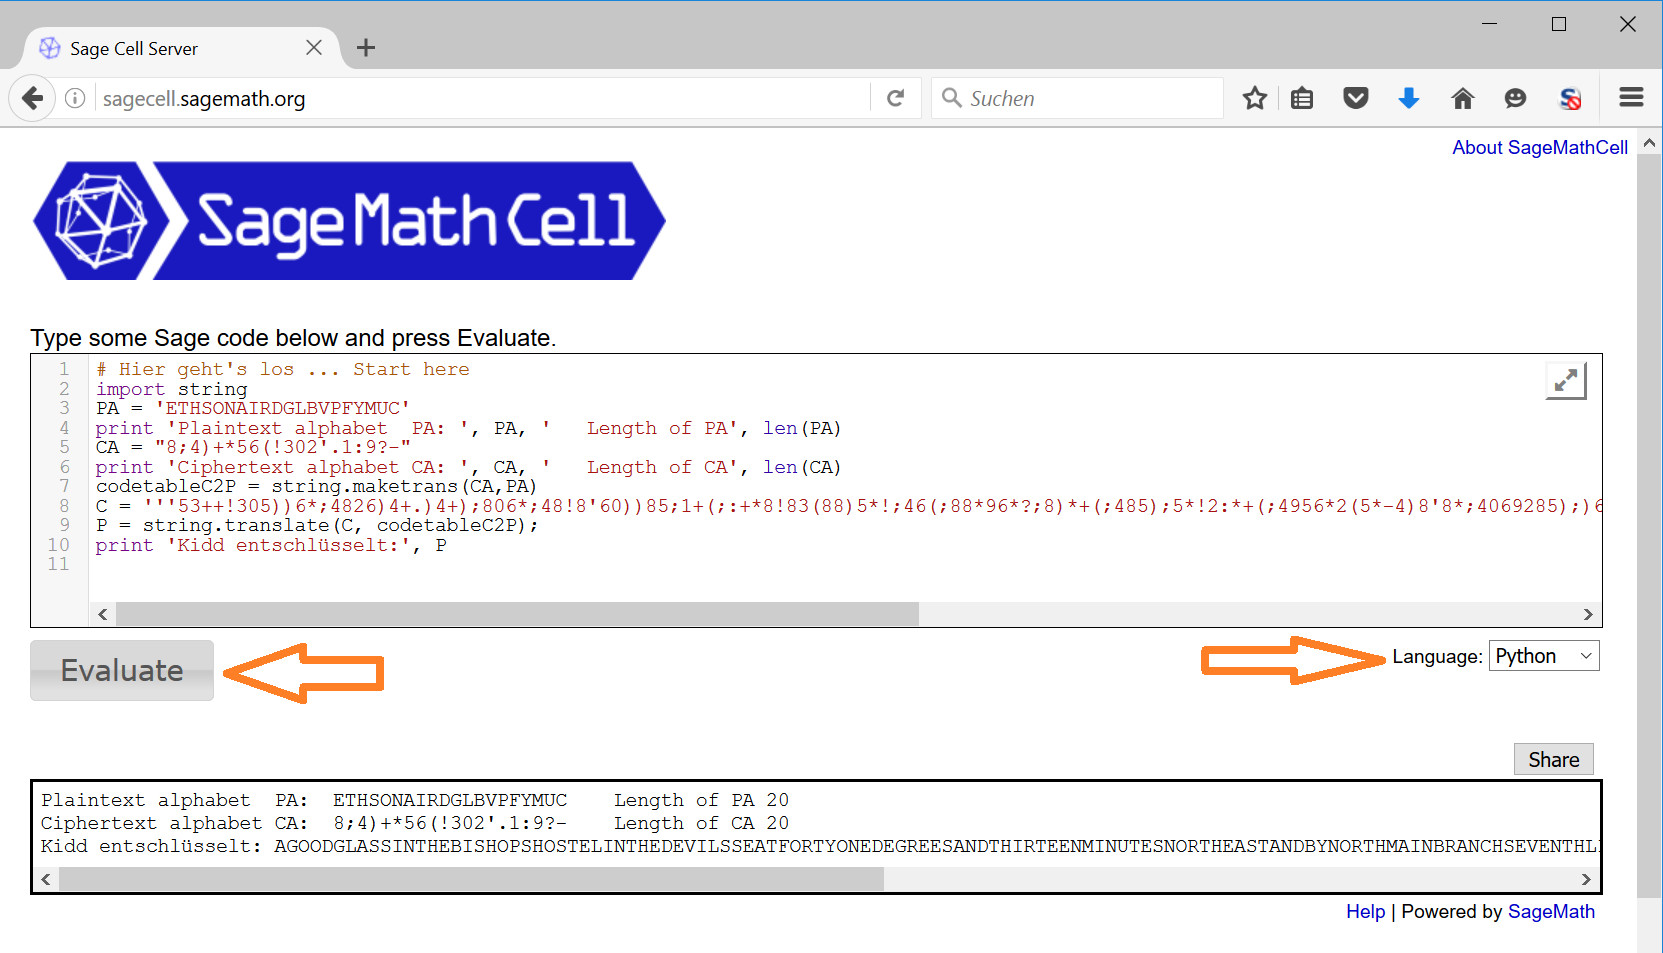
\includegraphics[scale=0.53]{../en/figures/Using-SageMathCell-with-Python-for-Poes-GoldBug}
\caption{Benutzung von SageMathCell, um Poes Goldkäfer zu entschlüsseln (mit Python\index{Python})}
\label{MOV_Using-SageMathCell-with-Python-for-Poes-GoldBug}
\end{center}
\end{figure}


\noindent Als Ergebnis erhalten wir:

% \noindent \verb muss auf derselben Zeile enden.
\begin{Verbatim}%

Plaintext alphabet  PA:  ETHSONAIRDGLBVPFYMUC    Length of PA 20
Ciphertext alphabet CA:  8;4)+*56(!302'.1:9?-    Length of CA 20
Kidd decrypted: AGOODGLASSINTHEBISHOPSHOSTELINTHEDEVILSSEATFORTYONEDEGREES
                ANDTHIRTEENMINUTESNORTHEASTANDBYNORTHMAINBRANCHSEVENTHLIMB
                EASTSIDESHOOTFROMTHELEFTEYEOFTHEDEATHSHEADABEELINEFROMTHE
                TREETHROUGHTHESHOTFIFTYFEETOUT

\end{Verbatim}

\noindent Man sieht gut, wie wenig Code man mit Python\index{Python} oder Sage für solche Aufgaben benötigt.
Im obigen Beispiel waren es 2 überflüssige Kommentarzeilen, 3 Zeilen Eingabe, 3 Zeilen echter Code und 3 Zeilen Ausgabe;
effektiv nötig waren 7 Zeilen Code.





% ++++++++++++++++++++++++++++++++++++++++++++++++++++++++++++++++++++++++++
\newpage
\hypertarget{appendix-Learn-NT}{}
\section{Lernprogramm Elementare Zahlentheorie}
    \label{s:appendix-Learn-NT}
    \index{ZT, Lernprogramm Zahlentheorie}%
    \index{Lernprogramm ZT}%

In CT1\index{CT1} ist ein interaktives Lernprogramm zur elementaren
{\em Zahlentheorie}, genannt "`ZT"', enthalten.\footnote{%
    ZT können Sie in CT1\index{CT1} über das Menü
    \textbf{Einzelverfahren \textbackslash{} Zahlentheorie
    interaktiv \textbackslash{} Lernprogramm für Zahlentheorie} aufrufen.
}

Das Lernprogramm "`NT"' (Zahlentheorie) von Martin Ramberger führt in die
Zahlentheorie ein und visualisiert viele der Verfahren und Konzepte.
Wo nötig zeigt es auch die entsprechenden mathematischen Formeln.
Oftmals können die mathematischen Verfahren dynamisch mit eigenen kleinen
Zahlenbeispielen ausprobiert werden.

Die Inhalte basieren vor allem auf den Büchern von
\cite{Buchmann2016} und \cite{Scheid2006}.

Dieses visualisierte Lernprogramm wurde mit Authorware 4 erstellt.\footnote{%
    Da Authorware veraltet ist und der Hersteller keine Portierungswerkzeuge
    auf seine Nachfolgeprodukte zur Verfügung stellte, wird das ZT-Programm
    nicht mehr weiter entwickelt.
}

\paragraph*{Bitte um Erweiterung/Upgrade:}
Ein Update auf die neueste Version von Authorware oder auf eine andere
Entwicklungsplattform wäre wünschenswert. Wenn sich hierzu Interessenten
finden, würde ich mich sehr freuen (bitte E-Mail an den Autor des
CrypTool-Skriptes).


\paragraph*{Abbildungen:}
Die Abbildungen~\ref{NT_Fig_C1.3_EuclidsAlg-LinearCombinations}
bis~\ref{NT_Fig_C5.3_PollardRho} vermitteln einen Eindruck des
Lernprogramms "`ZT"':


% -> Figur 1  WIE ERREICHT MAN, dass er von vorne zählt ? (nicht wichtig)
%
% \includegraphics[scale=0.5]{figures/NT_Fig_C1.3_EuclidsAlg-LinearCombinations}
%    geht nicht. Im Dateinamen darf keine Punkt sein !!!?????!!!!!
%    Die Dateiendung muss man weglassen.
%
\begin{figure}[ht]
\begin{center}
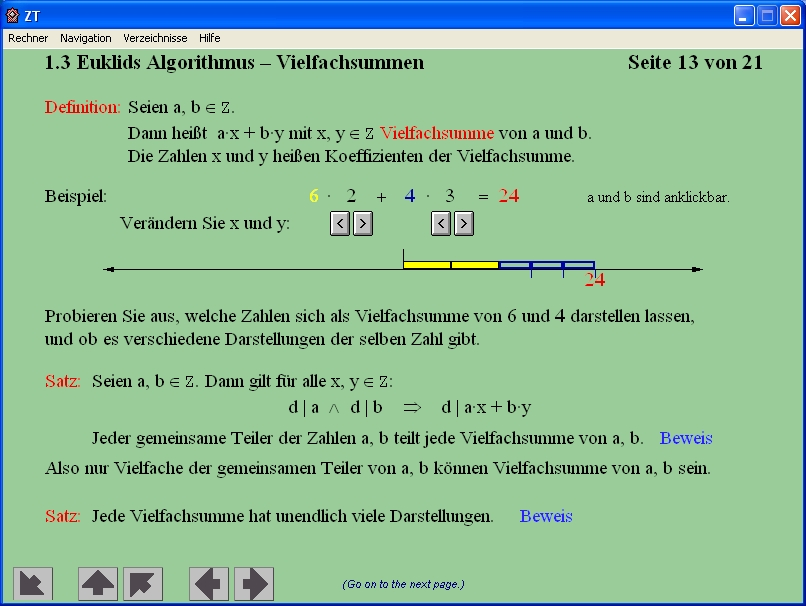
\includegraphics[scale=0.4]{figures/NT_Fig_C1-3_EuclidsAlg-LinearCombinations}
\caption{Jeder gemeinsame Teiler zweier Zahlen teilt auch alle ihre Linearkombinationen}
%%% TODO_Layout: Nur in Teilen von movies wird bei caption noch \vspace{1ex} hinzugefügt.
%%%              Damit sind die Abstände im Abbildungsverzeichnis von A.9 bis A.16
%%%              unterschiedlich vom Rest --> nahm es wieder raus. Analog wurde etwas
%%%              Platz unter den Abb-Untertitel in Kap. 7 geschaffen, der nun auch weg (22.8.16)
%%%              --> Wenn man es macht, dann muss man es überall machen!
%%% Bsp: vorher:  \caption{Euklids Algorithmus zur Bestimmung des ggT\vspace{1ex}}
%%%      nachher: \caption{Euklids Algorithmus zur Bestimmung des ggT}
\label{NT_Fig_C1.3_EuclidsAlg-LinearCombinations}
\end{center}
\end{figure}


\begin{figure}[ht]
\begin{center}
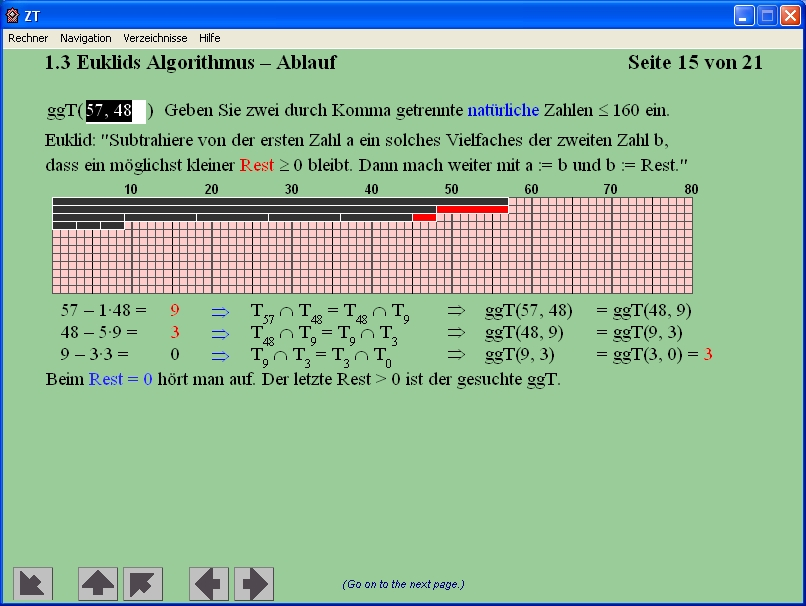
\includegraphics[scale=0.4]{figures/NT_Fig_C1-3_EuclidsAlg-Procedure}
\caption{Euklids Algorithmus zur Bestimmung des ggT}
\label{NT_Fig_C1.3_EuclidsAlg-Procedure}
\end{center}
\end{figure}


\begin{figure}[ht]
\begin{center}
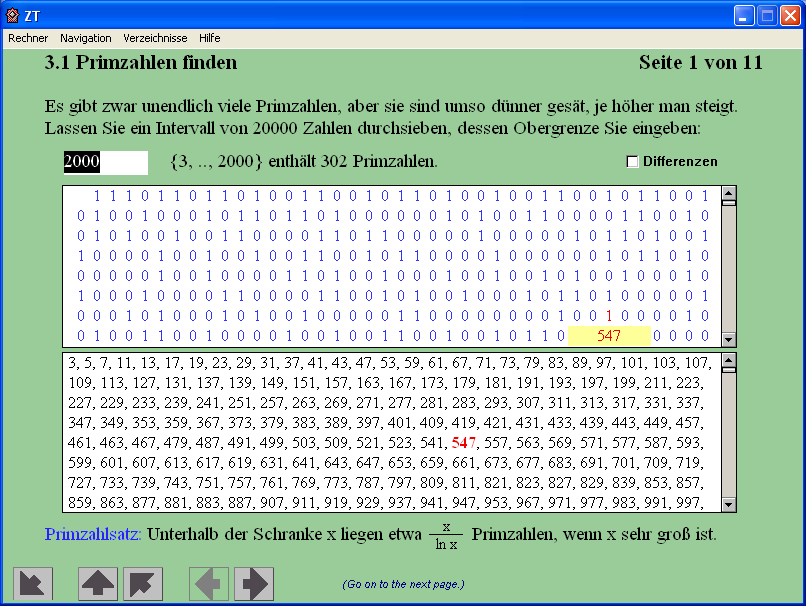
\includegraphics[scale=0.4]{figures/NT_Fig_C3-1_PrimesDistribution}
\caption{Verteilung der Primzahlen und ihrer Differenzen}
\label{NT_Fig_C3.1_PrimesDistribution}
\end{center}
\end{figure}


\begin{figure}[ht]
\begin{center}
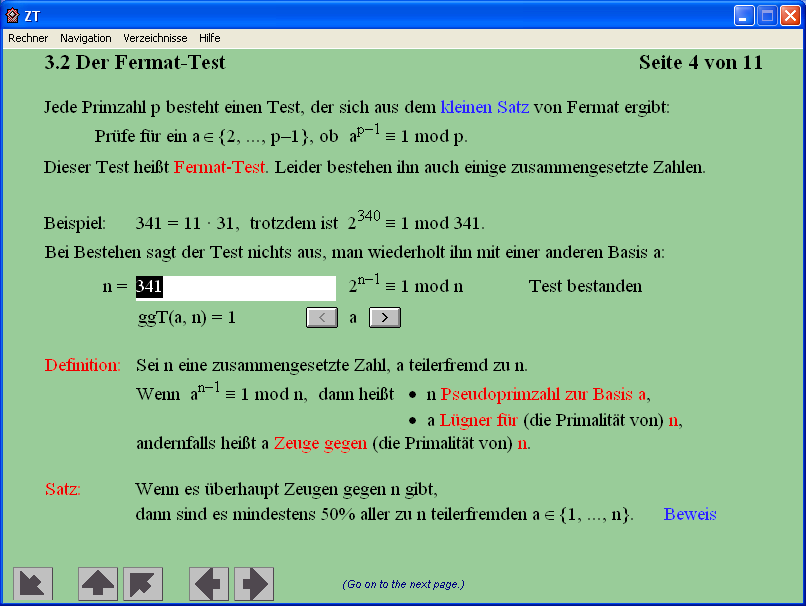
\includegraphics[scale=0.4]{figures/NT_Fig_C3-2_Fermat-Test}
\caption{Primzahlen finden mit dem Primzahltest nach Fermat}
\label{NT_Fig_C3.2_Fermat-Test}
\end{center}
\end{figure}


\begin{figure}[ht]
\begin{center}
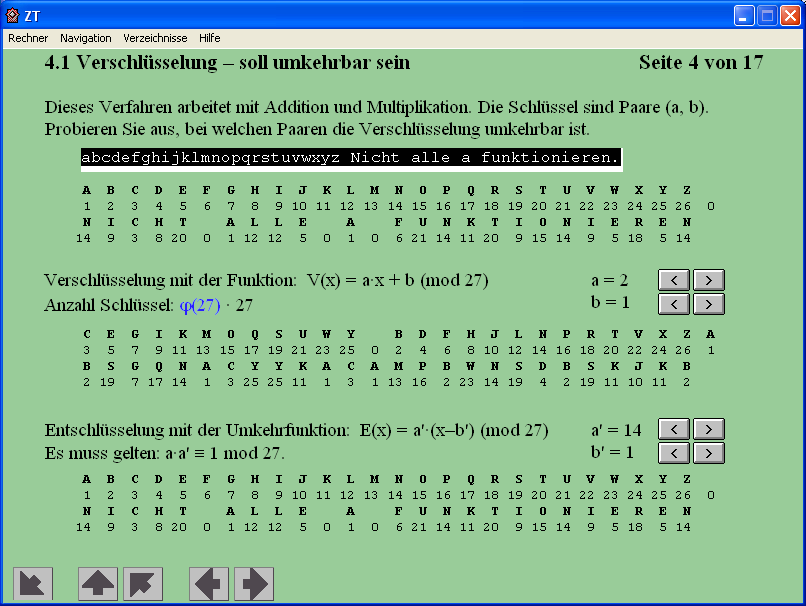
\includegraphics[scale=0.4]{figures/NT_Fig_C4-1_ReversibilityAdditiveCipher}
\caption{Umkehrbarkeit von Verschlüsselungsalgoritmen am Beispiel additiver Chiffren}
\label{NT_Fig_C4.1_ReversibilityAdditiveCipher}
\end{center}
\end{figure}


\begin{figure}[ht]
\begin{center}
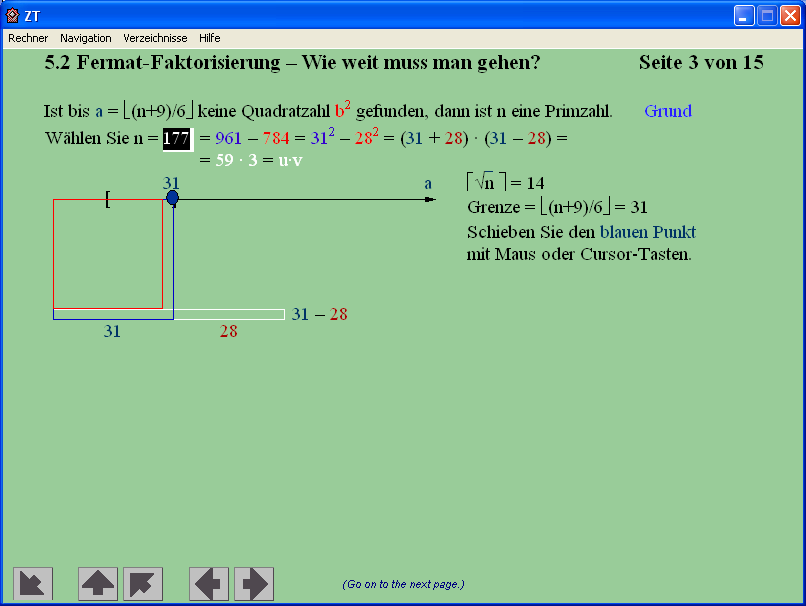
\includegraphics[scale=0.4]{figures/NT_Fig_C5-2_Fermat-factorization-How-far-1}
\caption{Fermat-Faktorisierung m.H. der 3. Binomischen Formel}
\label{NT_Fig_C5.2_Fermat-factorization-How-far-1}
\end{center}
\end{figure}


\begin{figure}[ht]
\begin{center}
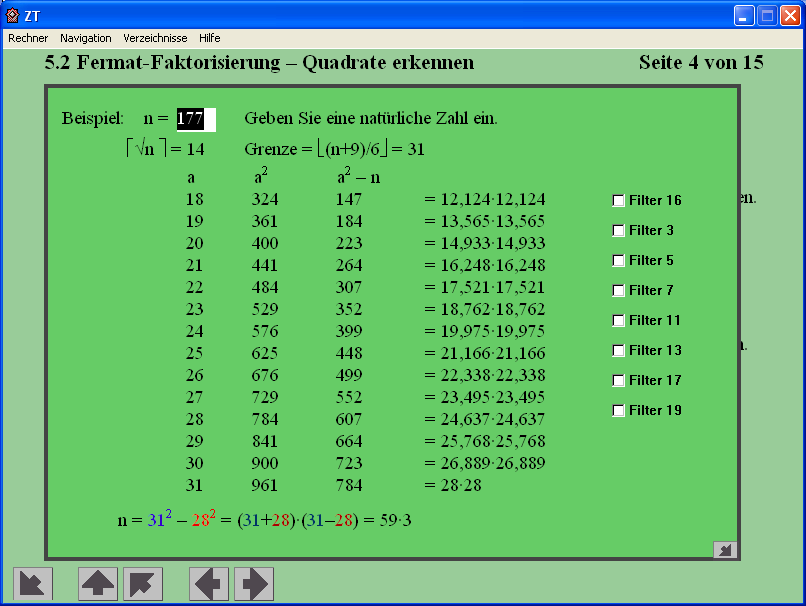
\includegraphics[scale=0.4]{figures/NT_Fig_C5-2_Fermat-factorization-How-far-2}
\caption{Fermat-Faktorisierung: Quadrate erkennen}
\label{NT_Fig_C5.2_Fermat-factorization-How-far-2}
\end{center}
\end{figure}


\begin{figure}[ht]
\begin{center}
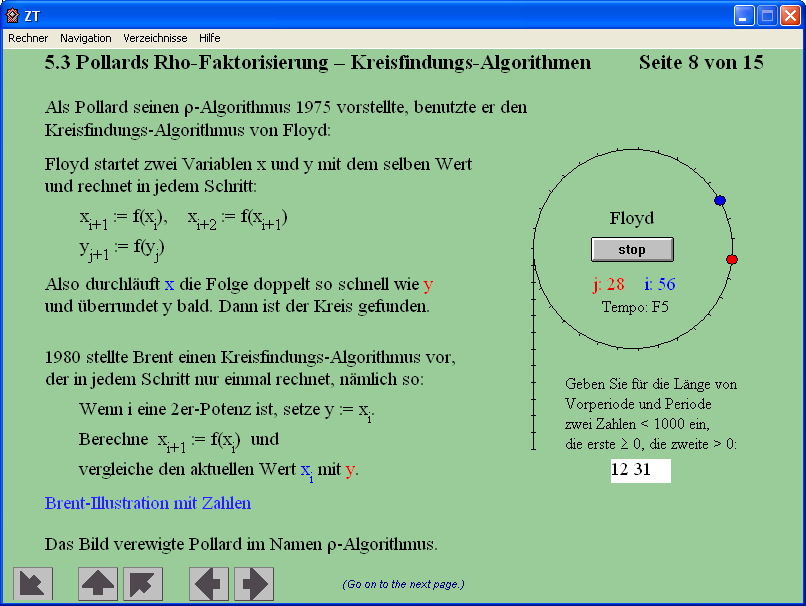
\includegraphics[scale=0.4]{figures/NT_Fig_C5-3_PollardRho}
\caption{Pollards Rho-Faktorisierung: Kreisfindungsalgorithmus nach Floyd}
\label{NT_Fig_C5.3_PollardRho}
\end{center}
\end{figure}



%------------------------------------------------------------------------------
\printbibliography[%
	heading=subbibintoc,
	title={Literatur zu Kapitel \thechapter},
	segment=\therefsegment,
]


\end{refsegment}
